\vspace{1.5cm}


En la figura~\figref{fig:fig_p8_maximun_load_for_regulation} se muestra el gráfico de la tensión en las entradas de la llave analógica en función de la resistencia de carga $R_{L}$, el gráfico se obtuvo realizando una simulación paramétrica, con el comando \textbf{SPICE} \textit{.step}, y luego se exportó el resultado y se procesó y graficó en \textbf{MATLAB}. En el gráfico se puede apreciar que está marcado el valor donde se cruzan los valores de tensión en las entradas de la llave, $1 \si[per-mode=symbol]{\volt}$, el valor de resistencia de carga al que se produce este cruce, se asumió como el valor de transición, el valor obtenido es de $4.88 \si[per-mode=symbol]{\ohm}$. Se graficó también en la misma escala la tensión de salida en función de la resistencia de carga, donde también se marcó el valor al que se produce la transición, se produce a un valor de tensión de salida de $9.81 \si[per-mode=symbol]{\volt}$, el valor nominal esperado es de $10 \si[per-mode=symbol]{\volt}$.


\vfill

\clearpage

\begin{figure}[H] %htb
\begin{center}
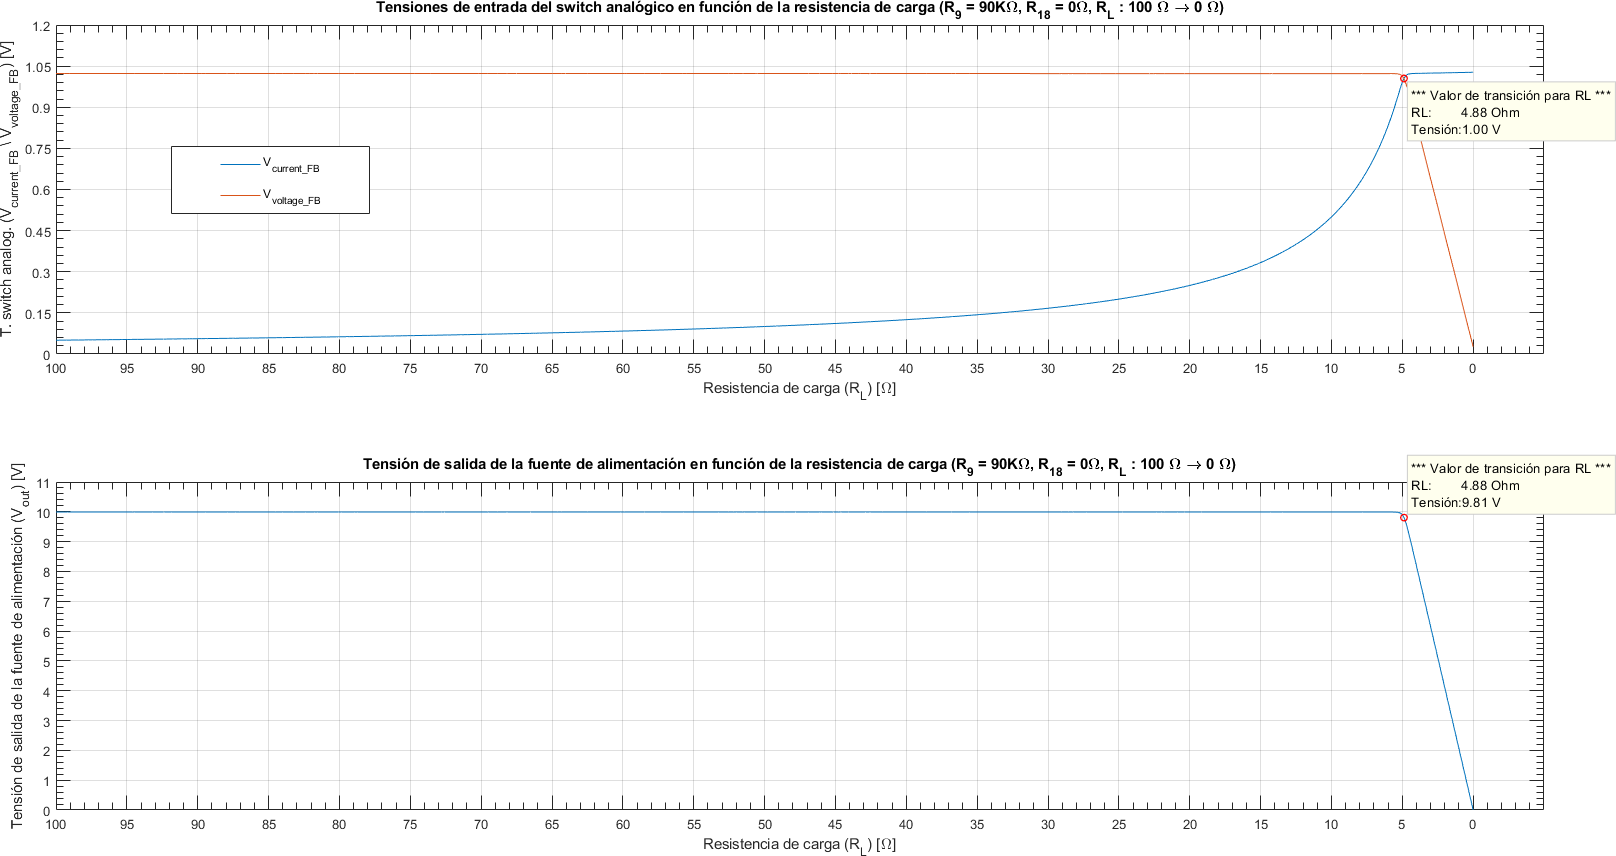
\includegraphics[width=1.1 \textwidth, angle=90]{./img/preguntas/p8.png}
\caption{\label{fig:fig_p8_maximun_load_for_regulation}\footnotesize{Tensión en las entradas del switch analógico y tensión de salida, en función de $R_{L}$, con esta variando entre $100 \si[per-mode=symbol]{\ohm}$ y $0 \si[per-mode=symbol]{\ohm}$.}}
\end{center}
\end{figure}



\clearpage